\chapter{Kiểm thử hệ thống}\label{chap:testing}
		Kiếm thử phần mềm là một việc rất quan trọng trong quy trình phát triển phần mềm.
        Để một hệ thống có thể đi vào hoạt động ổn định, các nhà phát triển cần kiểm tra tất
        cả tính năng, các thành phần của hệ thống, mọi thứ phải hoạt động một cách trơn tru
        mới có thể chuyển giao đến tay người sử dụng. Bất kỳ một lỗi nhỏ nào nếu không kiểm
        tra kỹ càng cũng có thể để lại hậu quả về sau, làm cho hệ thống không đáng tin cậy và
        không được sự hưởng ứng từ phía người dùng.
        
        Quy trình kiểm thử cần phải qua nhiều loại khác nhau: Unit test, Intergration test, System test, Acceptance test, Functional testing, Non Functional testing, End to end test... Hiện nay có rất nhiều thư viện kiểm thử hiệu quả và mạnh mẽ. Katalon Recorder là một extension dành cho chrome đã tích hợp tính năng kiểm thử vào trong nó để kiểm thử chức năng. Jmeter là công cụ để đo độ tải và performance của trang web và nhóm đã sử dụng K6 cloud platform có tích hợp jmeter để có thể kiểm thử phi chức năng cho trang web của nhóm.
		\section{Kiểm thử API}
		Đối với hệ thống nhóm xây dựng, các thành phần giao tiếp với nhau thông qua API. Vì vậy, cần phải kiểm thử riêng biệt các API trước khi tích hợp vào các bên. Nhóm chọn phần mềm Postman để kiểm thử các API.\\
		
		\textbf{API đăng nhập}
		
		\begin{figure}[!ht]
			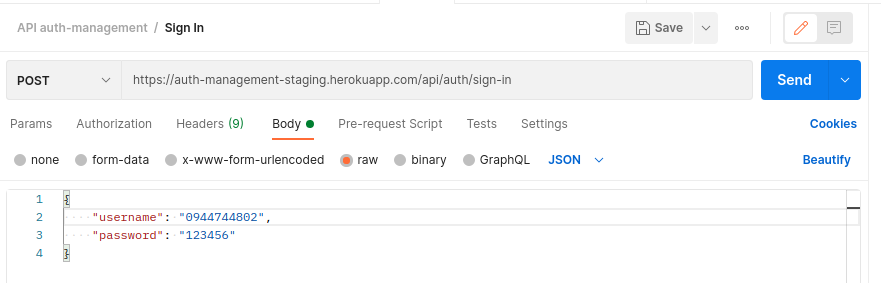
\includegraphics[width=0.8\textwidth]{Images/testing/API-sign-in.png}
			\centering
			\linebreak
			\caption{Kiểm thử với API đăng nhập}
		\end{figure}
		
		\newpage

		\begin{figure}[!ht]
			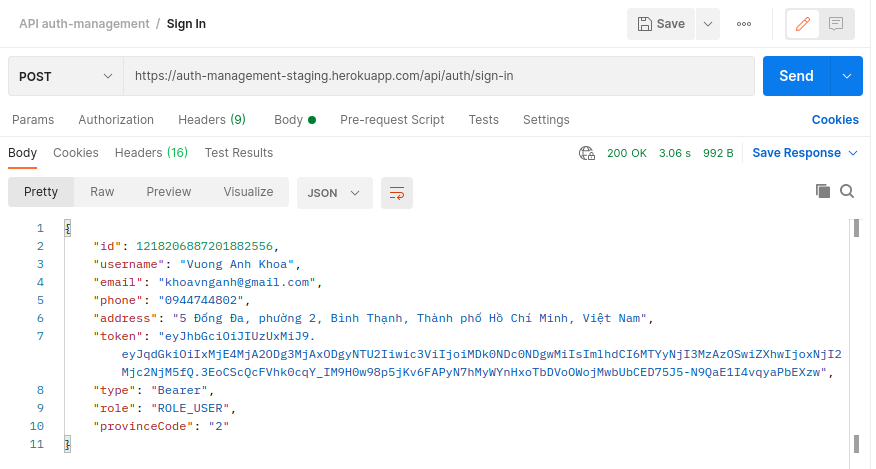
\includegraphics[width=0.8\textwidth]{Images/testing/API-sign-in-result.png}
			\centering
			\linebreak
			\caption{Kết quả kiểm thử với API đăng nhập}
		\end{figure}
		
		\newpage	
		
		\textbf{API đăng ký}
		
		\begin{figure}[!ht]
			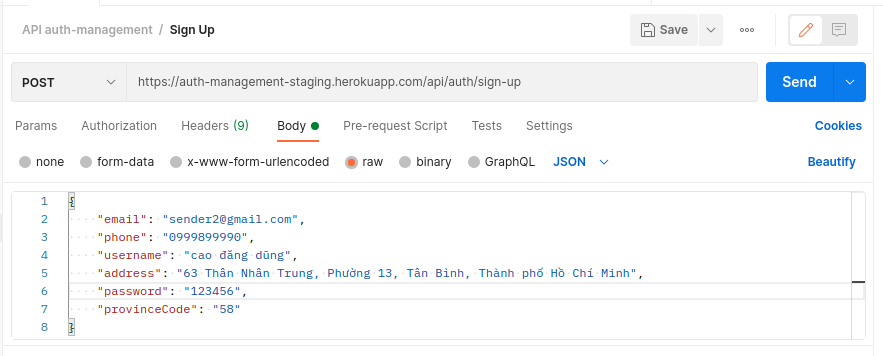
\includegraphics[width=0.8\textwidth]{Images/testing/API-sign-up.png}
			\centering
			\linebreak
			\caption{Kiểm thử với API đăng ký}
		\end{figure}
		
		\begin{figure}[!ht]
			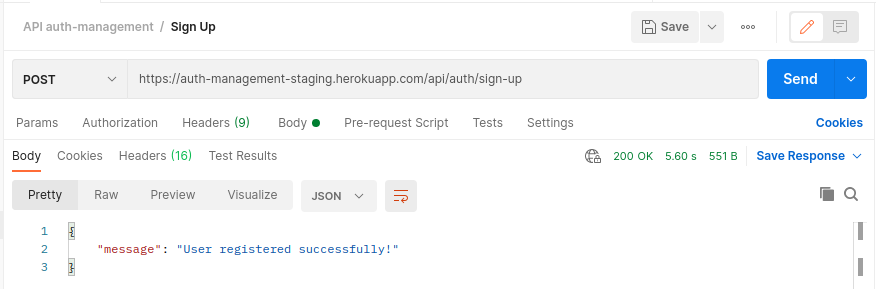
\includegraphics[width=0.8\textwidth]{Images/testing/API-sign-up-result.png}
			\centering
			\linebreak
			\caption{Kết quả kiểm thử với API đăng ký}
		\end{figure}
		
		\newpage
		
		\textbf{API thêm kho}
		
		\begin{figure}[!ht]
			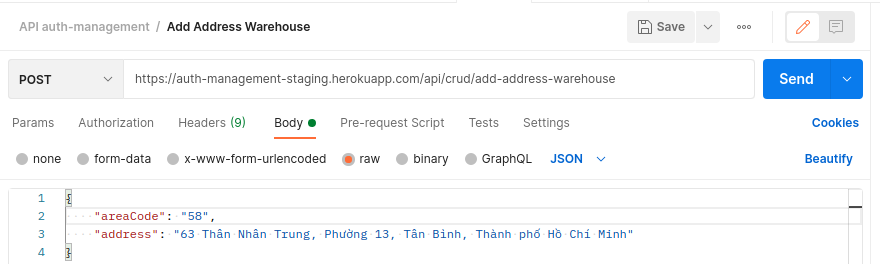
\includegraphics[width=0.8\textwidth]{Images/testing/API-add-address-warehouse.png}
			\centering
			\linebreak
			\caption{Kiểm thử với API thêm kho}
		\end{figure}
		
		\begin{figure}[!ht]
			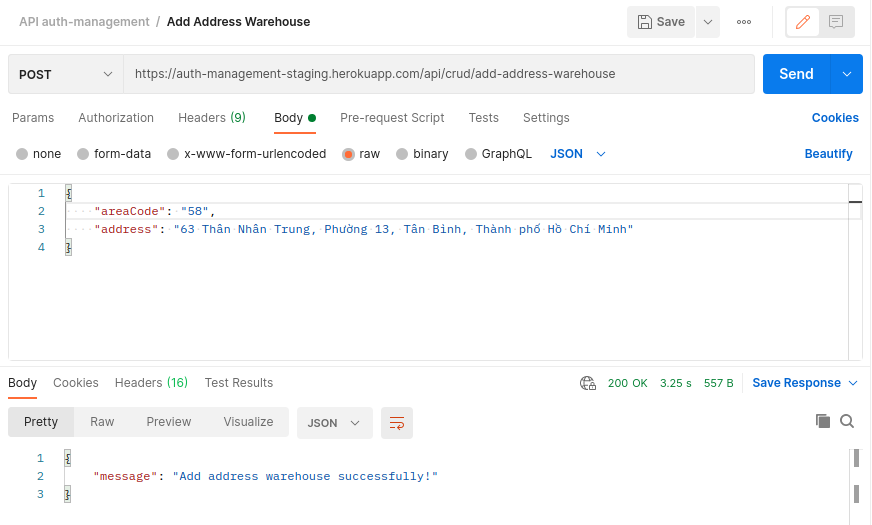
\includegraphics[width=0.8\textwidth]{Images/testing/API-add-address-warehouse-result.png}
			\centering
			\linebreak
			\caption{Kết quả kiểm thử với API thêm kho}
		\end{figure}
		
		\newpage	
		
		\textbf{API thêm tài xế}
		
		\begin{figure}[!ht]
			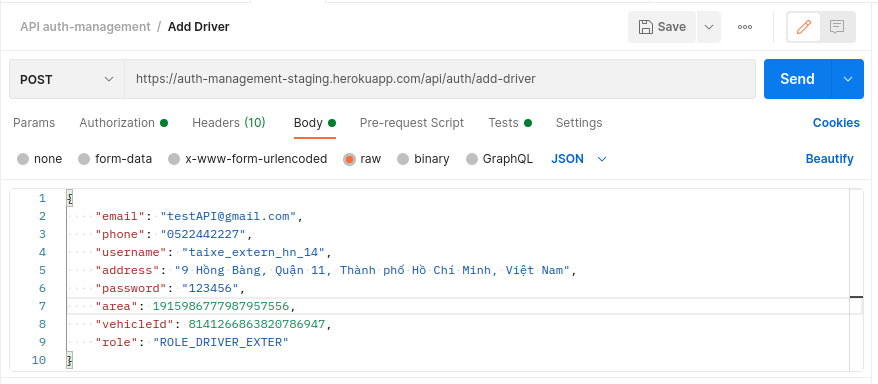
\includegraphics[width=0.8\textwidth]{Images/testing/API-add-driver.png}
			\centering
			\linebreak
			\caption{Kiểm thử với API thêm tài xế}
		\end{figure}
		
		\begin{figure}[!ht]
			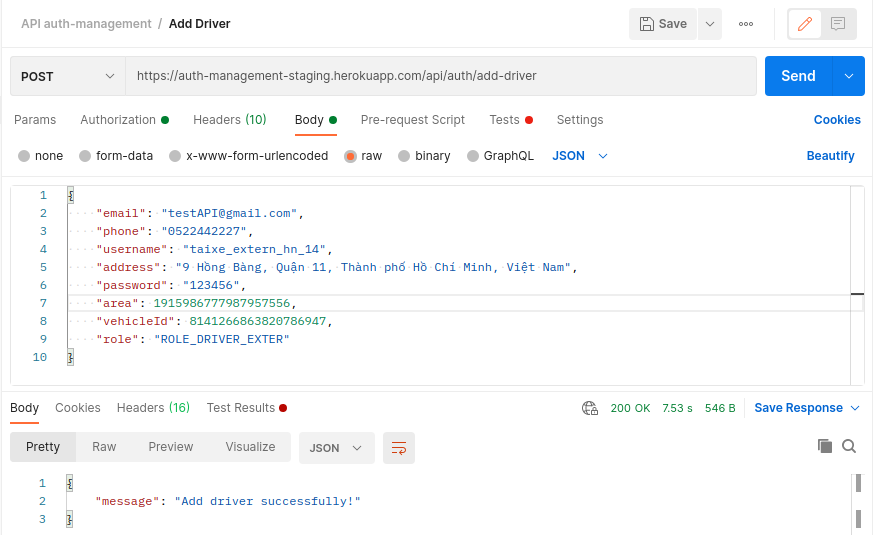
\includegraphics[width=0.8\textwidth]{Images/testing/API-add-driver-result.png}
			\centering
			\linebreak
			\caption{Kết quả kiểm thử với API thêm tài xế}
		\end{figure}
		
		\newpage
		
		\textbf{API thêm thủ kho}
		
		\begin{figure}[!ht]
			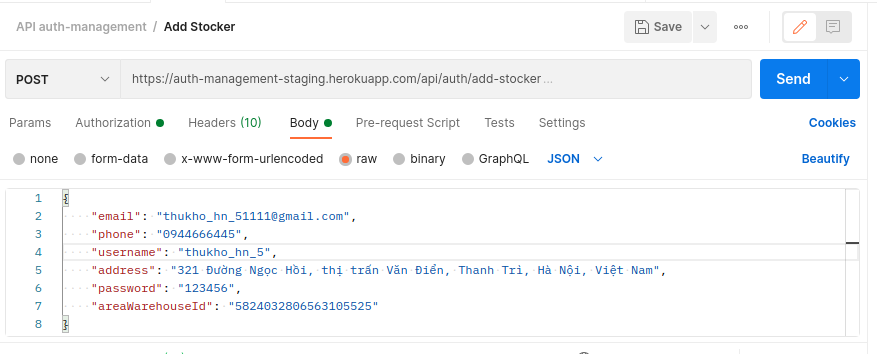
\includegraphics[width=0.8\textwidth]{Images/testing/API-add-stocker.png}
			\centering
			\linebreak
			\caption{Kiểm thử với API thêm thủ kho}
		\end{figure}
		
		\begin{figure}[!ht]
			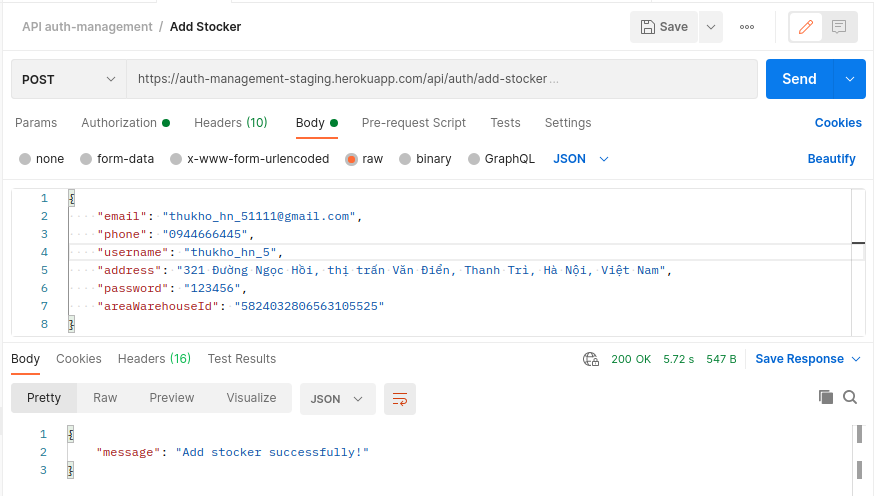
\includegraphics[width=0.8\textwidth]{Images/testing/API-add-stocker-result.png}
			\centering
			\linebreak
			\caption{Kết quả kiểm thử với API thêm thủ kho}
		\end{figure}
		
		\newpage
		
		\textbf{API thêm phương tiện}
		
		\begin{figure}[!ht]
			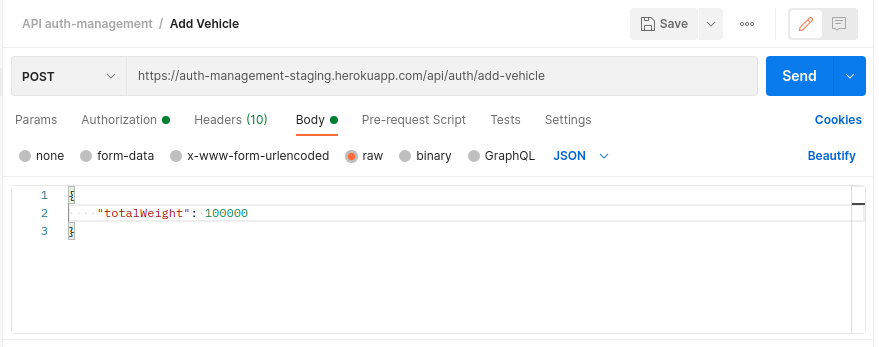
\includegraphics[width=0.8\textwidth]{Images/testing/API-add-vehicle.png}
			\centering
			\linebreak
			\caption{Kiểm thử với API thêm phương tiện}
		\end{figure}
		
		\begin{figure}[!ht]
			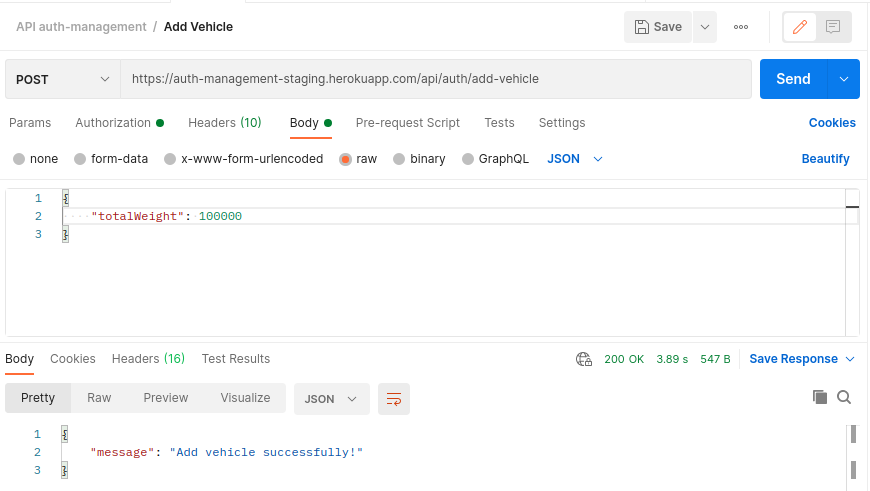
\includegraphics[width=0.8\textwidth]{Images/testing/API-add-vehicle-result.png}
			\centering
			\linebreak
			\caption{Kết quả kiểm thử với API thêm phương tiện}
		\end{figure}
		
		\newpage
		
		\textbf{API đổi mât khẩu}
		
		\begin{figure}[!ht]
			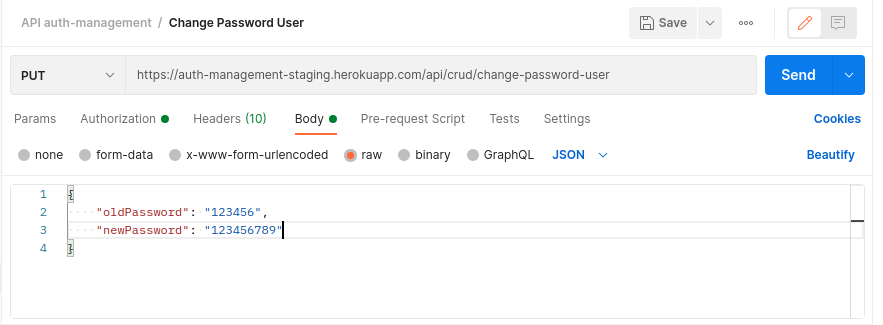
\includegraphics[width=0.8\textwidth]{Images/testing/API-change-password.png}
			\centering
			\linebreak
			\caption{Kiểm thử với API đổi mật khẩu}
		\end{figure}
		
		\begin{figure}[!ht]
			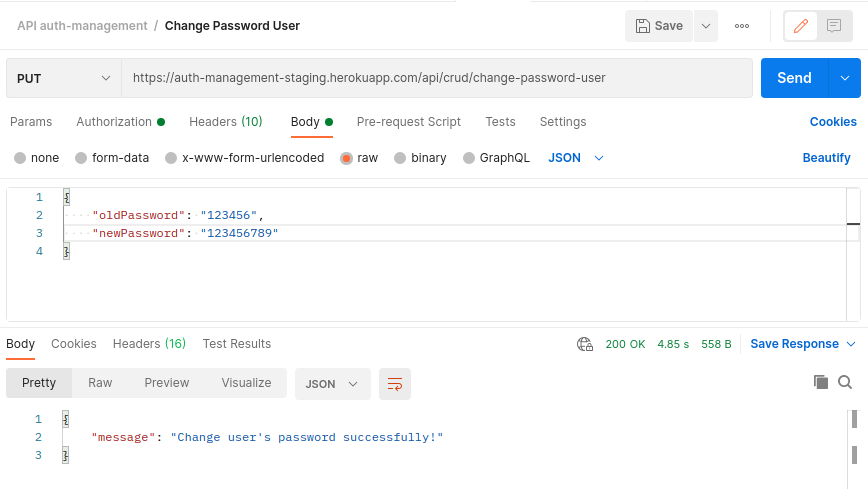
\includegraphics[width=0.8\textwidth]{Images/testing/API-change-password-result.png}
			\centering
			\linebreak
			\caption{Kết quả kiểm thử với API đổi mât khẩu}
		\end{figure}
		
		\newpage
		
		\textbf{API lấy phí vận chuyển}
		
		\begin{figure}[!ht]
			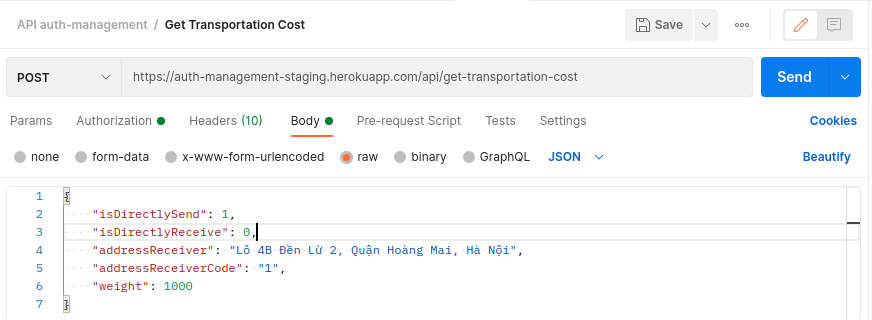
\includegraphics[width=0.8\textwidth]{Images/testing/API-get-cost.png}
			\centering
			\linebreak
			\caption{Kiểm thử với API lấy phí vận chuyển}
		\end{figure}
		
		\begin{figure}[!ht]
			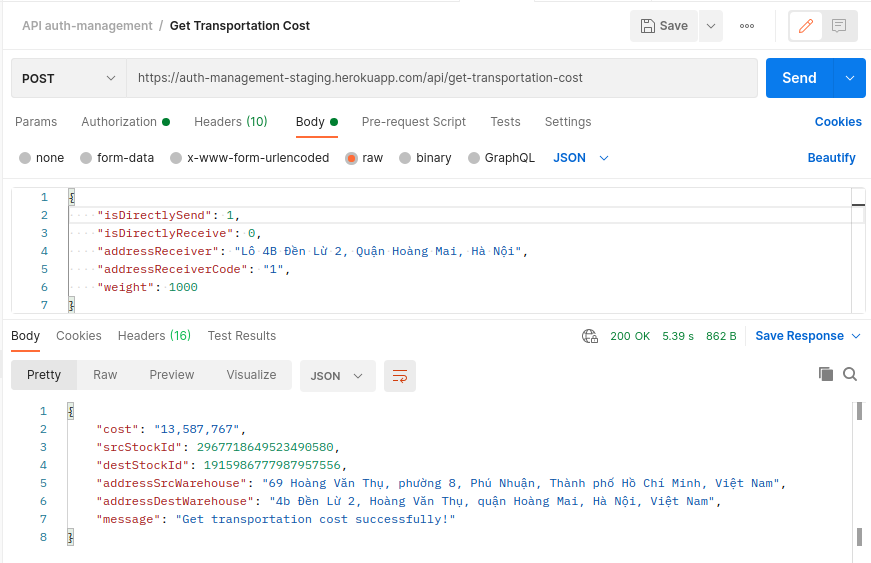
\includegraphics[width=0.8\textwidth]{Images/testing/API-get-cost-result.png}
			\centering
			\linebreak
			\caption{Kết quả kiểm thử với API lấy phí vận chuyển}
		\end{figure}
		
		\newpage
		
		\textbf{API lấy tài xế liên tỉnh ở kho}
		
		\begin{figure}[!ht]
			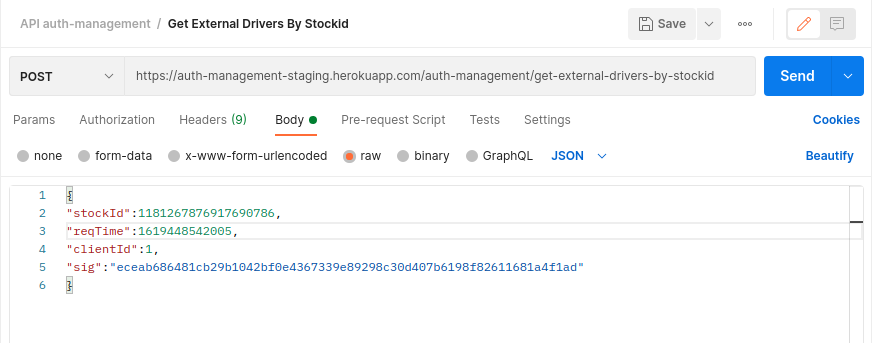
\includegraphics[width=0.8\textwidth]{Images/testing/API-get-driver-external-warehouse.png}
			\centering
			\linebreak
			\caption{Kiểm thử với API lấy tài xế liên tỉnh ở kho}
		\end{figure}
		
		\begin{figure}[!ht]
			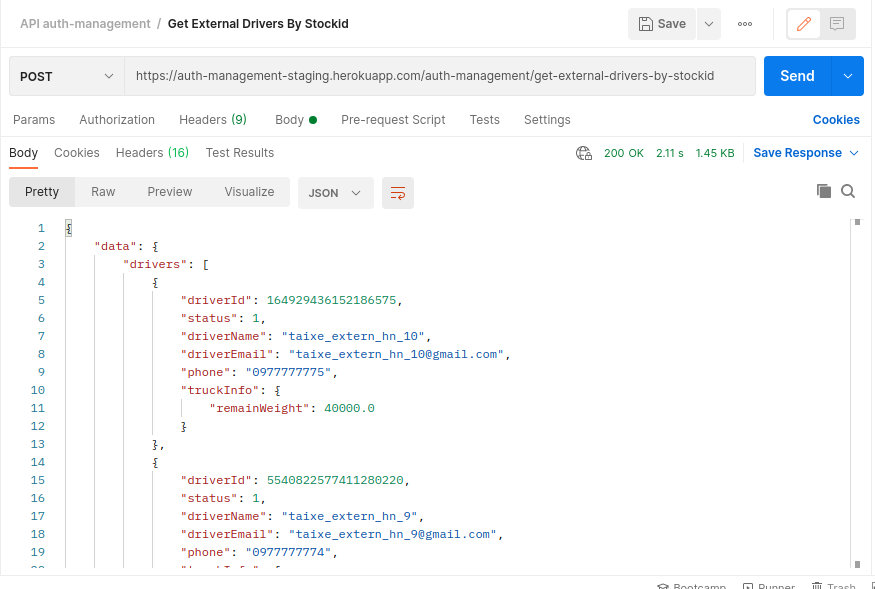
\includegraphics[width=0.8\textwidth]{Images/testing/API-get-driver-external-warehouse-result.png}
			\centering
			\linebreak
			\caption{Kết quả kiểm thử với API lấy tài xế liên tỉnh ở kho}
		\end{figure}
		
		\newpage
		
		\textbf{API lấy thông tin tài xế}
		
		\begin{figure}[!ht]
			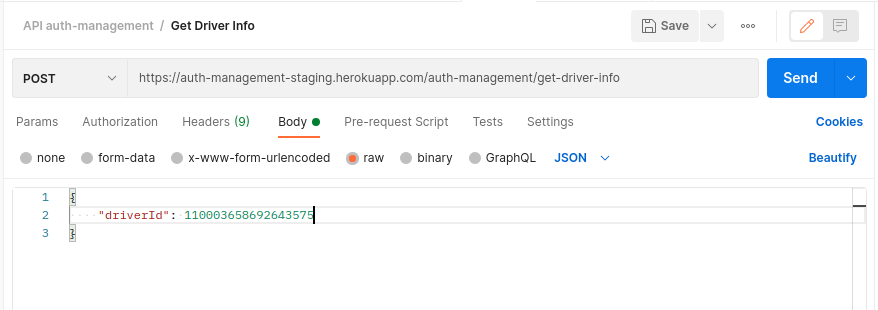
\includegraphics[width=0.8\textwidth]{Images/testing/API-get-driver-info.png}
			\centering
			\linebreak
			\caption{Kiểm thử với API lấy thông tin tài xế}
		\end{figure}
		
		\begin{figure}[!ht]
			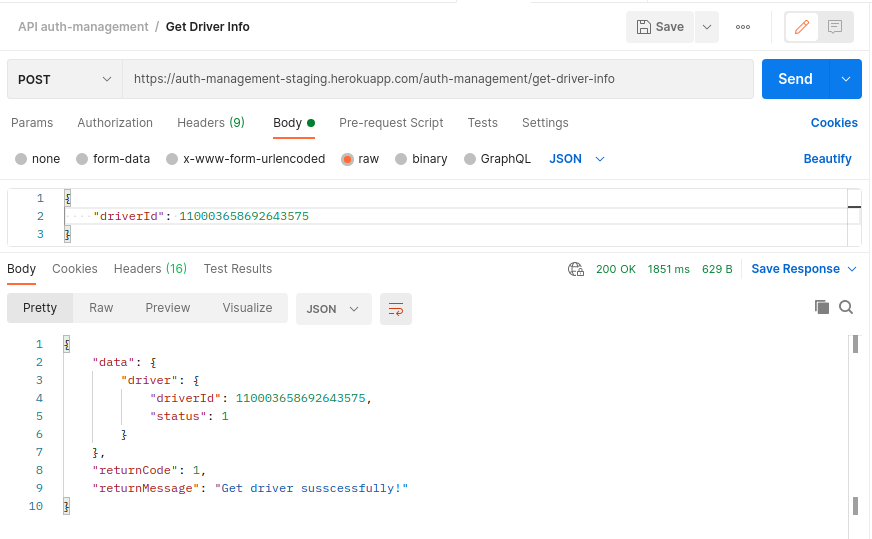
\includegraphics[width=0.8\textwidth]{Images/testing/API-get-driver-info-result.png}
			\centering
			\linebreak
			\caption{Kết quả kiểm thử với API lấy thông tin tài xế liên}
		\end{figure}
		
		\newpage
		
		\textbf{API lấy danh sách tài xế ở kho}
		
		\begin{figure}[!ht]
			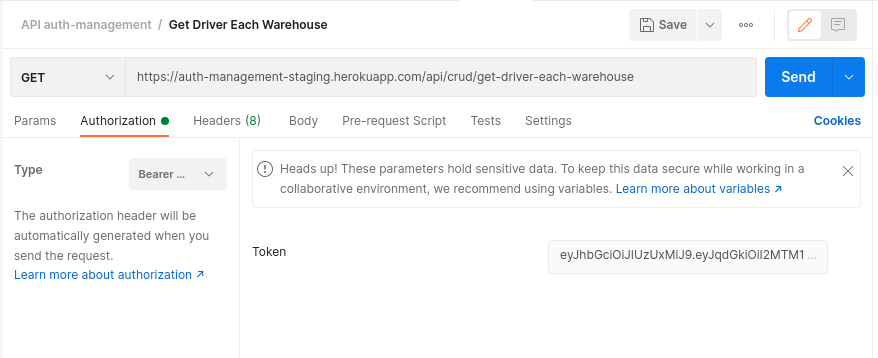
\includegraphics[width=0.8\textwidth]{Images/testing/API-get-driver-warehouse.png}
			\centering
			\linebreak
			\caption{Kiểm thử với API lấy danh sách tài xế ở kho}
		\end{figure}
		
		\begin{figure}[!ht]
			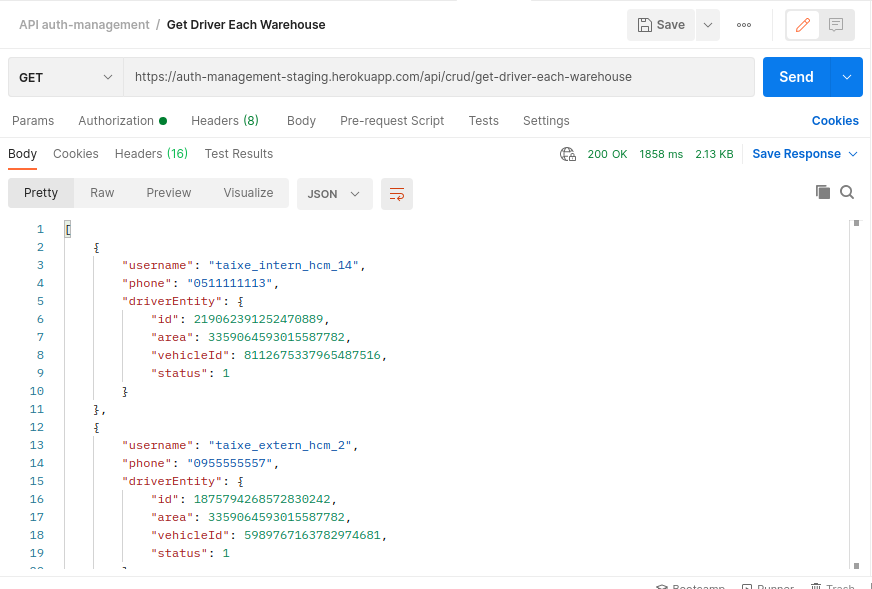
\includegraphics[width=0.8\textwidth]{Images/testing/API-get-driver-warehouse-result.png}
			\centering
			\linebreak
			\caption{Kết quả kiểm thử với API lấy danh sách tài xế ở kho}
		\end{figure}
		
		\newpage
		
		\textbf{API lấy danh sách tài xế}
		
		\begin{figure}[!ht]
			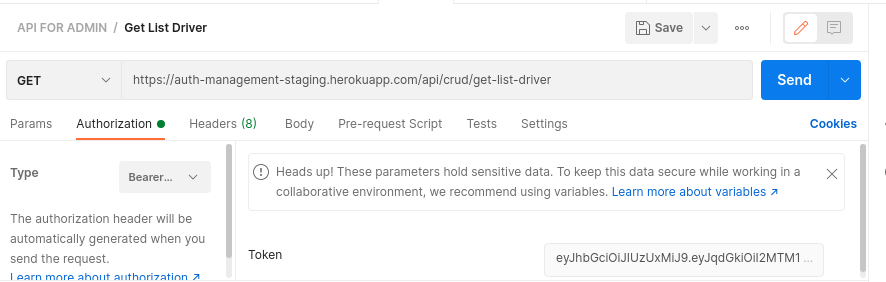
\includegraphics[width=0.8\textwidth]{Images/testing/API-get-list-drivers.png}
			\centering
			\linebreak
			\caption{Kiểm thử với API lấy danh sách tài xế}
		\end{figure}
		
		\begin{figure}[!ht]
			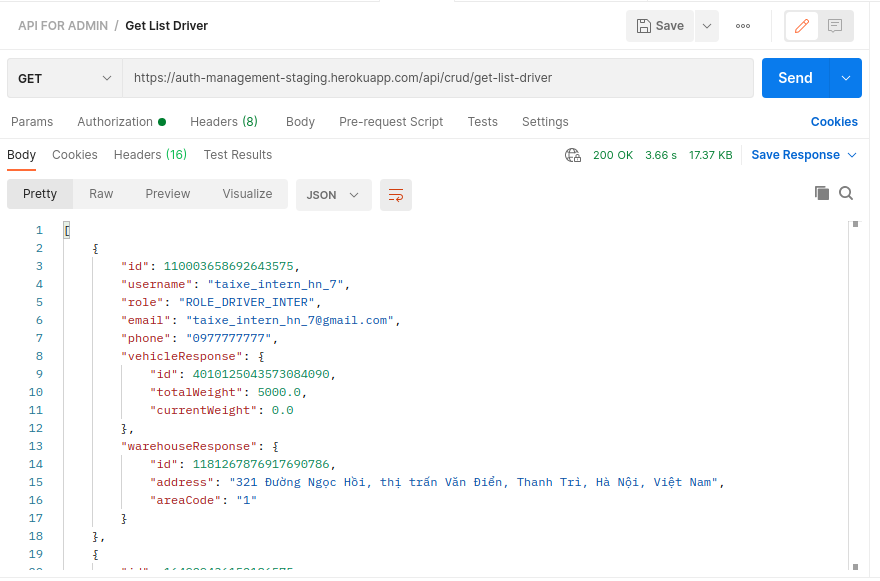
\includegraphics[width=0.8\textwidth]{Images/testing/API-get-list-drivers-result.png}
			\centering
			\linebreak
			\caption{Kết quả kiểm thử với API lấy danh sách tài xế}
		\end{figure}
		
		\newpage
		
		\textbf{API lấy danh sách thủ kho}
		
		\begin{figure}[!ht]
			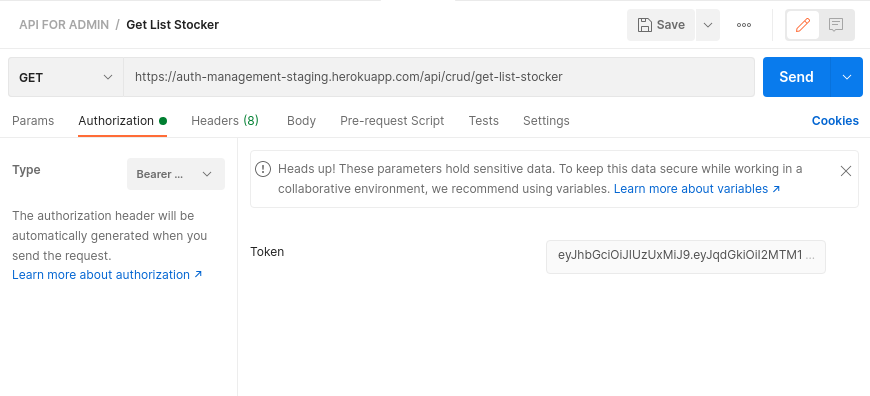
\includegraphics[width=0.8\textwidth]{Images/testing/API-get-list-stocker.png}
			\centering
			\linebreak
			\caption{Kiểm thử với API lấy danh sách thủ kho}
		\end{figure}
		
		\begin{figure}[!ht]
			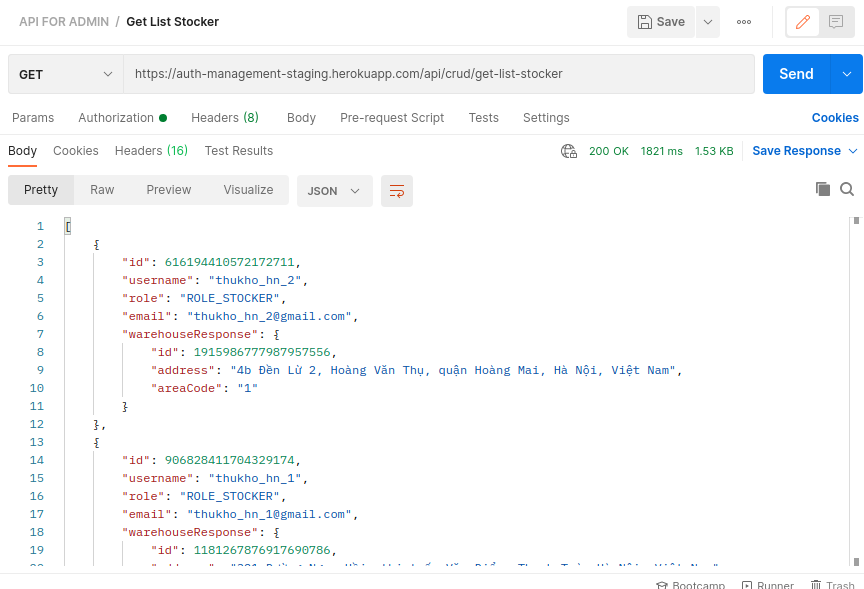
\includegraphics[width=0.8\textwidth]{Images/testing/API-get-list-stocker-result.png}
			\centering
			\linebreak
			\caption{Kết quả kiểm thử với API lấy danh sách thủ kho}
		\end{figure}
		
		\newpage
		
		\textbf{API lấy danh sách kho}
		
		\begin{figure}[!ht]
			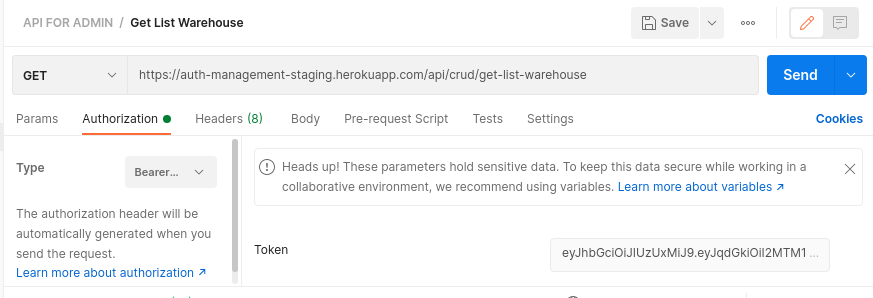
\includegraphics[width=0.8\textwidth]{Images/testing/API-get-list-warehouse.png}
			\centering
			\linebreak
			\caption{Kiểm thử với API lấy danh sách kho}
		\end{figure}
		
		\begin{figure}[!ht]
			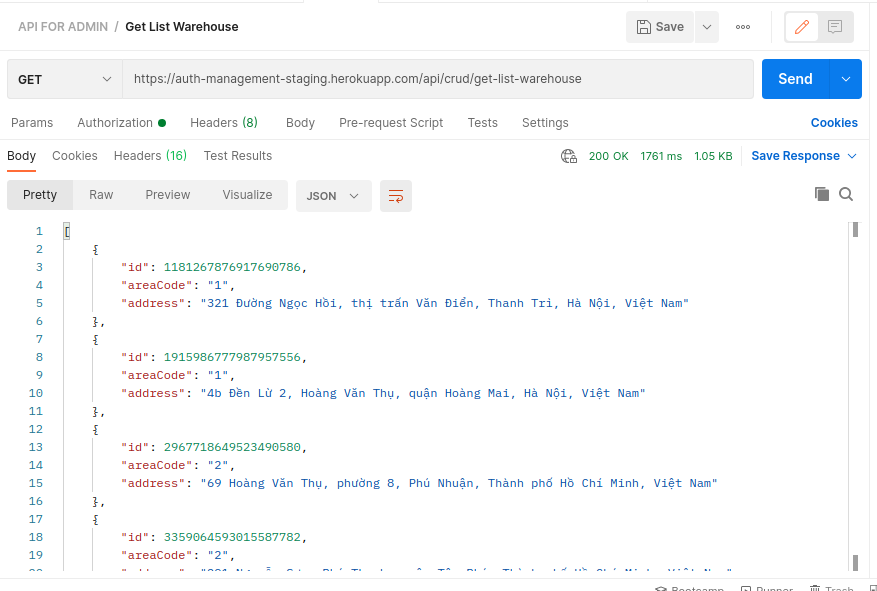
\includegraphics[width=0.8\textwidth]{Images/testing/API-get-list-warehouse-result.png}
			\centering
			\linebreak
			\caption{Kết quả kiểm thử với API lấy danh sách kho}
		\end{figure}
		
		\newpage
		
		\textbf{API lấy thông tin người dùng}
		
		\begin{figure}[!ht]
			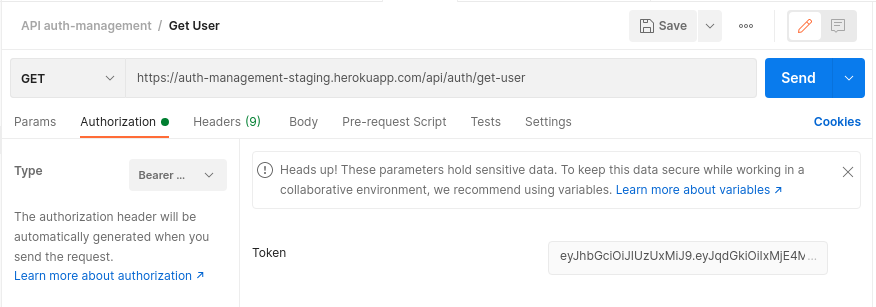
\includegraphics[width=0.8\textwidth]{Images/testing/API-get-user.png}
			\centering
			\linebreak
			\caption{Kiểm thử với API lấy thông tin người dùng}
		\end{figure}
		
		\begin{figure}[!ht]
			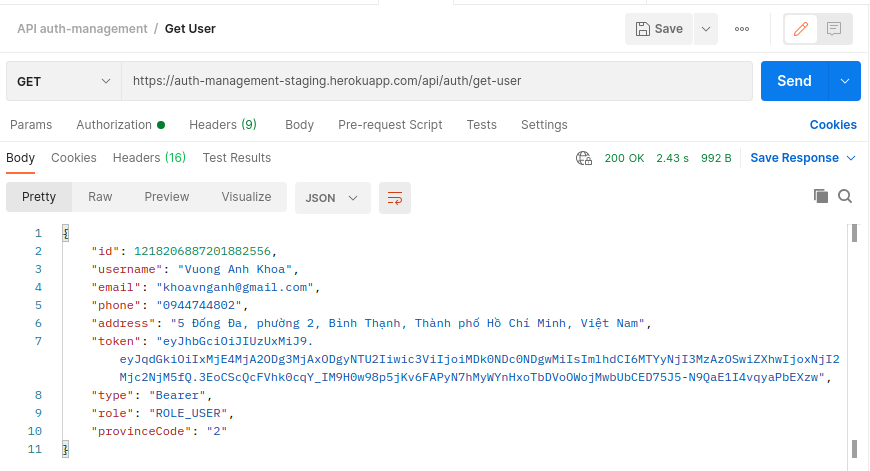
\includegraphics[width=0.8\textwidth]{Images/testing/API-get-user-result.png}
			\centering
			\linebreak
			\caption{Kết quả kiểm thử với API lấy thông tin người dùng}
		\end{figure}
		
		\newpage
		
		\textbf{API lấy danh sách phương tiện chưa sử dụng}
		
		\begin{figure}[!ht]
			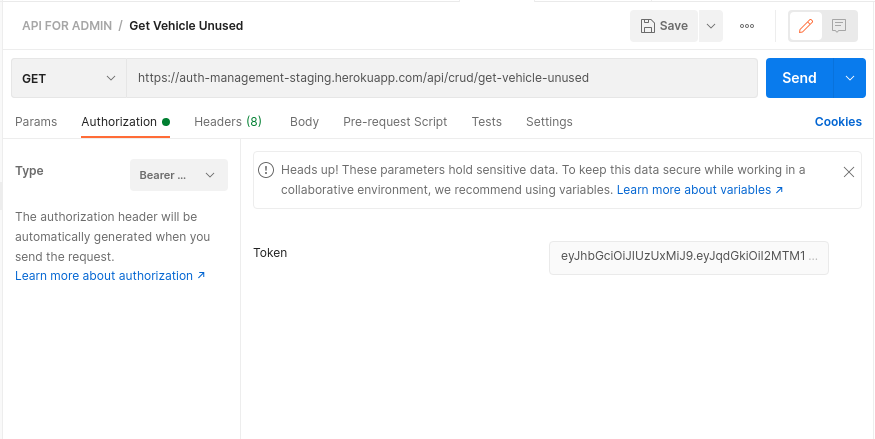
\includegraphics[width=0.8\textwidth]{Images/testing/API-get-vehicle-unused.png}
			\centering
			\linebreak
			\caption{Kiểm thử với API lấy danh sách phương tiện chưa sử dụng}
		\end{figure}
		
		\begin{figure}[!ht]
			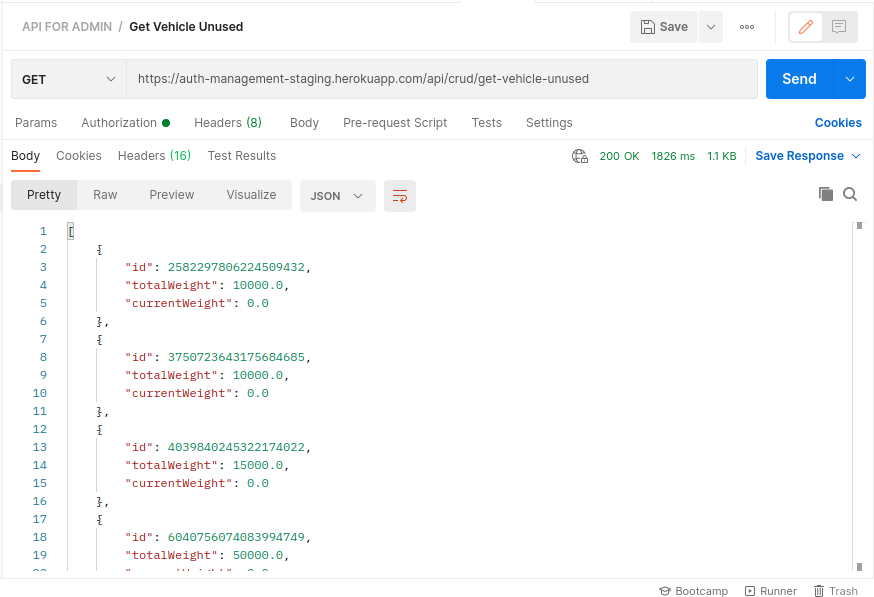
\includegraphics[width=0.8\textwidth]{Images/testing/API-get-vehicle-unused-result.png}
			\centering
			\linebreak
			\caption{Kết quả kiểm thử với API lấy danh sách phương tiện chưa sử dụng}
		\end{figure}
		
		\newpage
		
		\textbf{API cập nhật thông tin người dùng}
		
		\begin{figure}[!ht]
			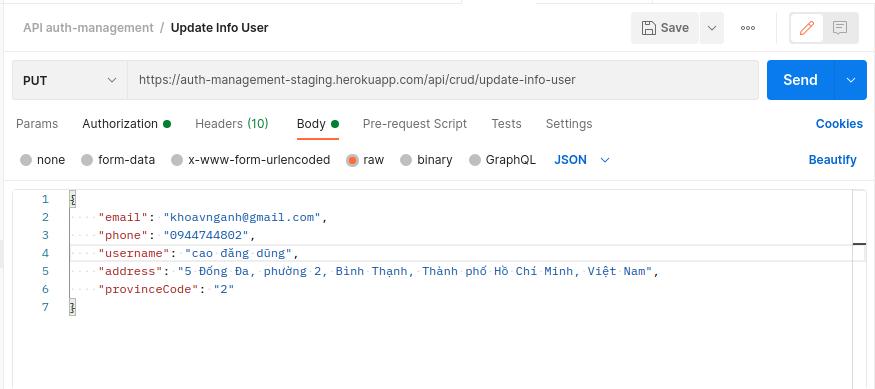
\includegraphics[width=0.8\textwidth]{Images/testing/API-update-info-user.png}
			\centering
			\linebreak
			\caption{Kiểm thử với API cập nhật thông tin người dùng}
		\end{figure}
		
		\begin{figure}[!ht]
			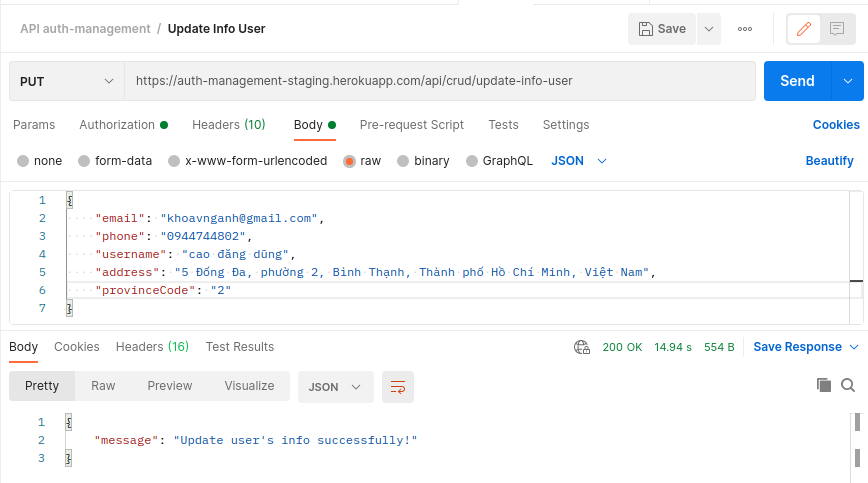
\includegraphics[width=0.8\textwidth]{Images/testing/API-update-info-user-result.png}
			\centering
			\linebreak
			\caption{Kết quả kiểm thử với API cập nhật thông tin người dùng}
		\end{figure}
		
		\newpage
		
		\textbf{API cập nhật trạng thái tài xế}
		
		\begin{figure}[!ht]
			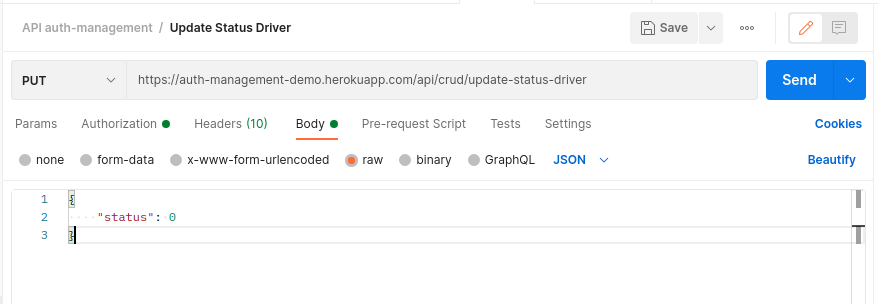
\includegraphics[width=0.8\textwidth]{Images/testing/API-update-status-driver.png}
			\centering
			\linebreak
			\caption{Kiểm thử với API cập nhật trạng thái tài xế}
		\end{figure}
		
		\begin{figure}[!ht]
			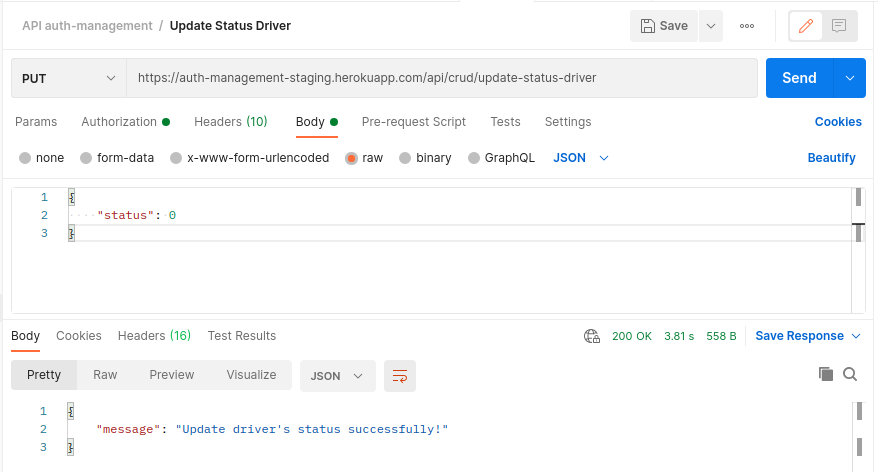
\includegraphics[width=0.8\textwidth]{Images/testing/API-update-status-driver-result.png}
			\centering
			\linebreak
			\caption{Kết quả kiểm thử với API cập nhật trạng thái tài xế}
		\end{figure}
		
		\newpage
		\section{Kiểm thử chức năng}
		    Vì tính chất nghiệp vụ có nhiều vai trò cũng như chức năng của các vai trò đó của trang web nên nhóm đã sử dụng Katalon Recorder để có thể kiểm thử tự động theo luồng các chức năng cơ bản của hệ thống.
			
		\section{Kiểm thử phi chức năng}
		    Kiểm thử phi chức năng (Non-functional testing) là kiểm tra một ứng dụng hoặc hệ thống phần mềm cho các yêu cầu phi chức năng của nó: cách thức hoạt động của một hệ thống, thay vì các hành vi cụ thể của hệ thống đó. Có rất nhiều loại kiểm thử phi chức năng như: performance test, baseline test, stress test... Đối với hệ thống của nhóm, nhóm sẽ tiến hành kiểm thử tải (load test). Kiểm tra tải là loại kiểm thử đề cập đến việc mô hình hóa sử dụng dự kiến của một hệ thống bằng cách mô phỏng nhiều người dùng truy cập hệ thống đồng thời.
		    
		    Nhóm sẽ sử dụng K6 cloud platform để tiến hành xây dựng kiểm thử với API đăng nhập:
		    https://auth-management-staging.osc-fr1.scalingo.io/api/auth/sign-in
		    
		Hình ảnh kiểm thử:
        
        \begin{figure}[!ht]
			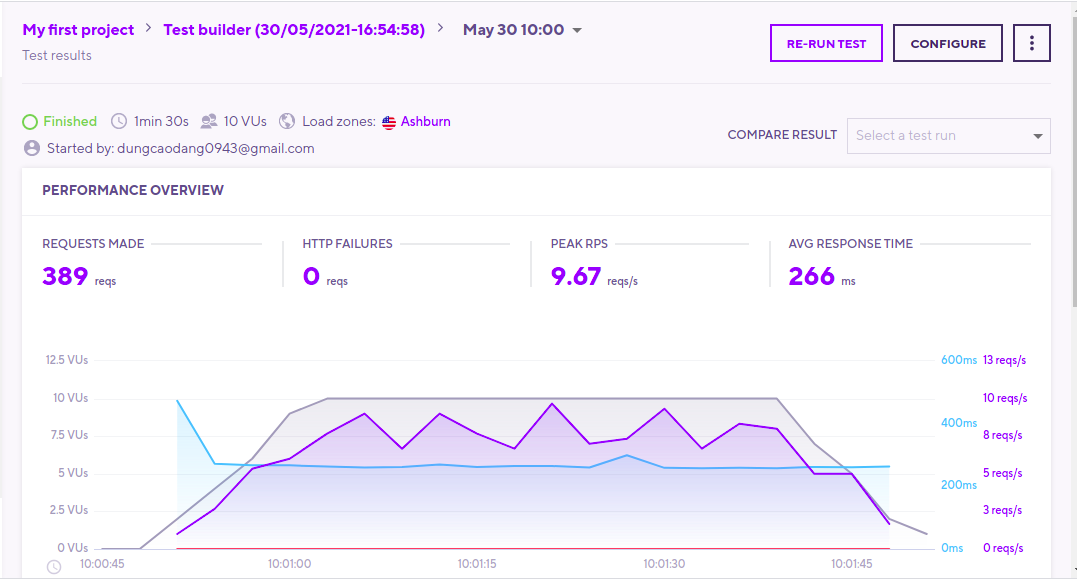
\includegraphics[width=0.8\textwidth]{Images/testing/testing_10.png}
			\centering
			\linebreak
			\caption{Kiểm thử với 10 users đồng thời}
		\end{figure}
	\newpage
		\begin{figure}[!ht]
			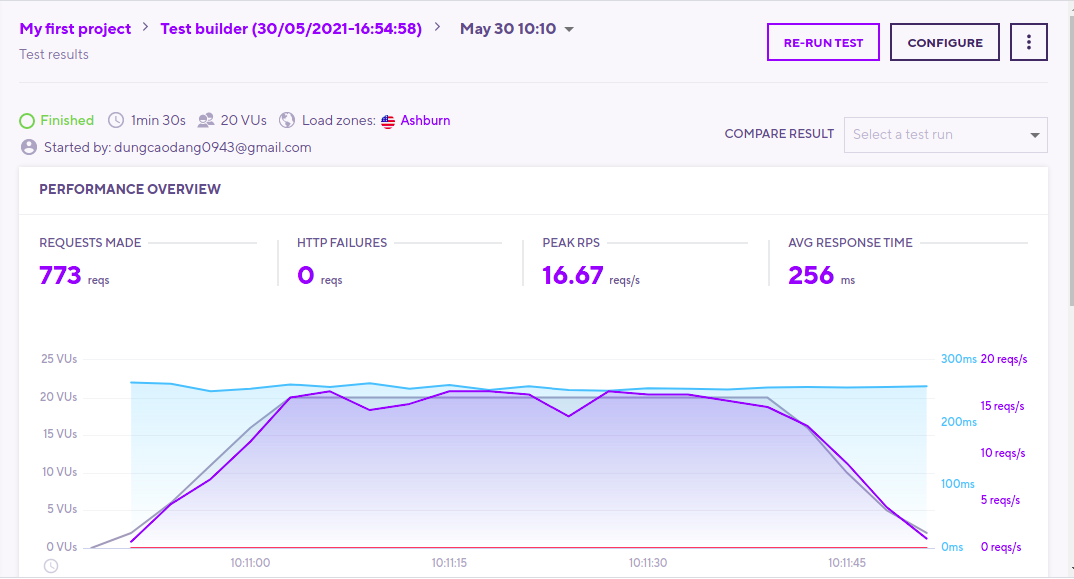
\includegraphics[width=0.8\textwidth]{Images/testing/testing_20.png}
			\centering
			\linebreak
			\caption{Kiểm thử với 20 users đồng thời}
		\end{figure}
		\newpage
		\begin{figure}[!ht]
			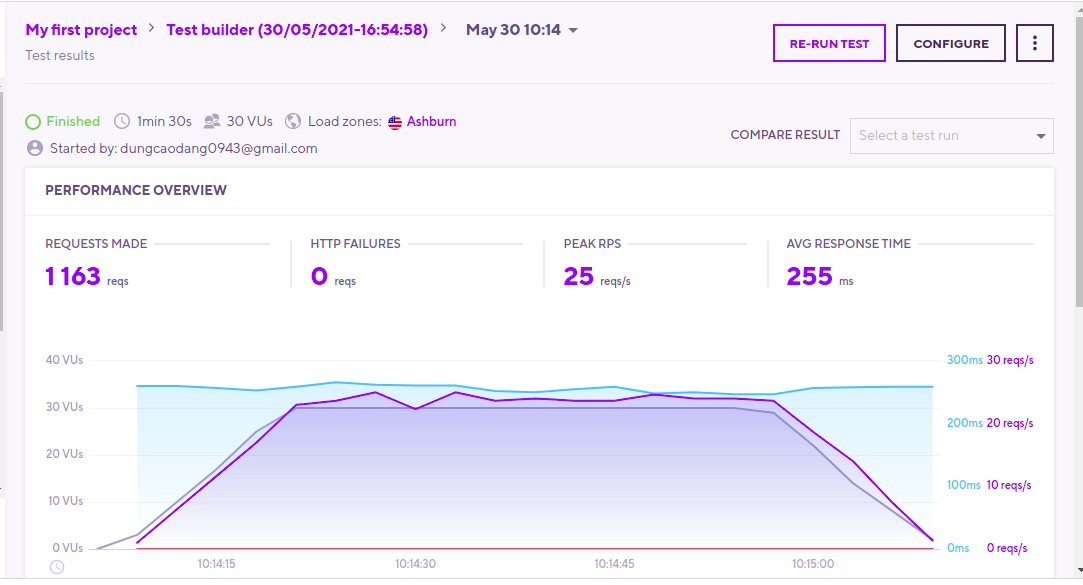
\includegraphics[width=0.8\textwidth]{Images/testing/testing_30.png}
			\centering
			\linebreak
			\caption{Kiểm thử với 30 users đồng thời}
		\end{figure}
		\begin{figure}[!ht]
			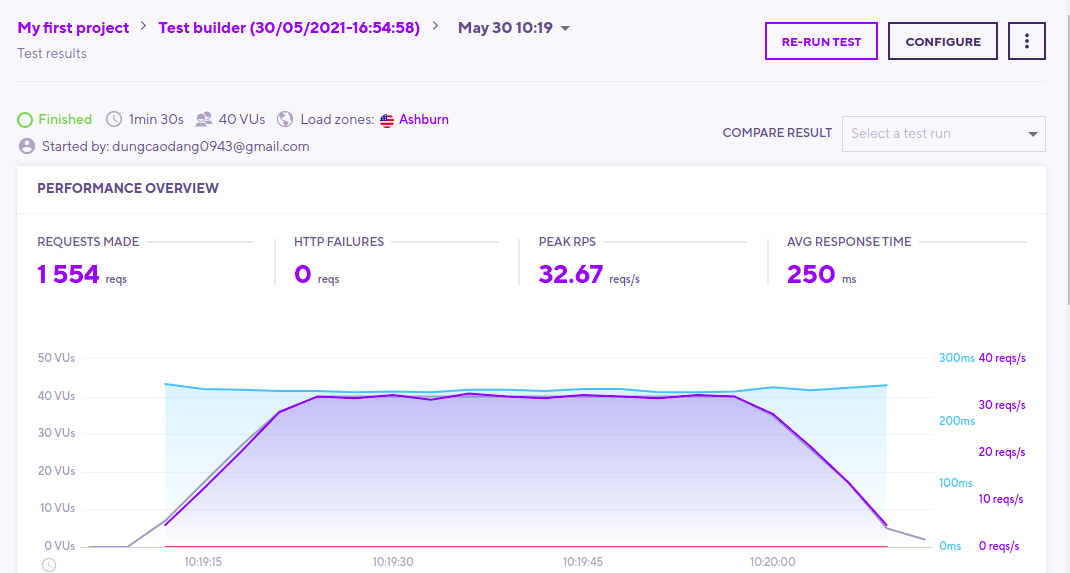
\includegraphics[width=0.8\textwidth]{Images/testing/testing_40.png}
			\centering
			\linebreak
			\caption{Kiểm thử với 40 users đồng thời}
		\end{figure}
	\newpage
		\begin{figure}[!ht]
			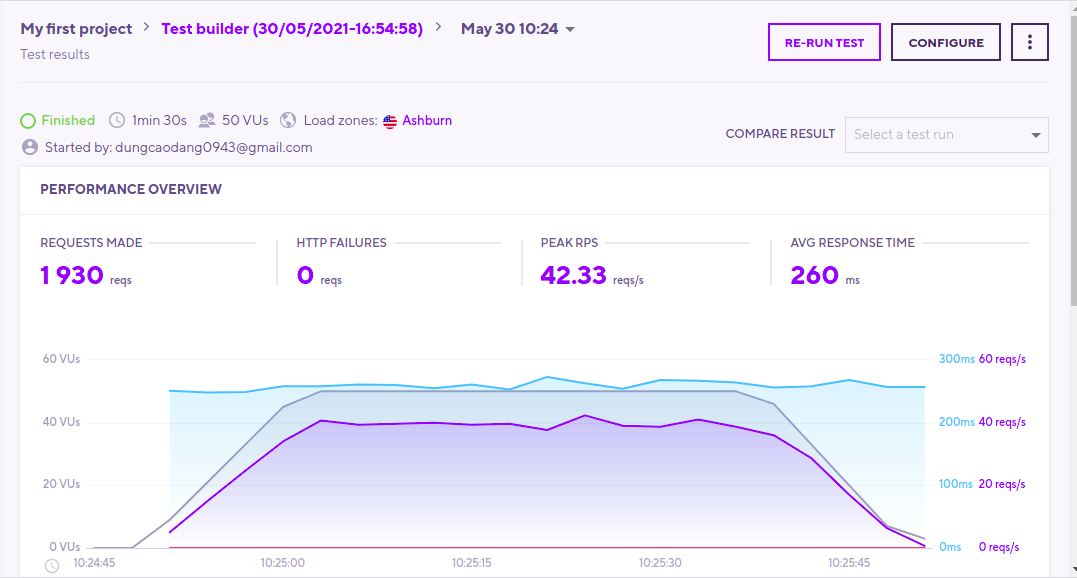
\includegraphics[width=0.8\textwidth]{Images/testing/testing_50.png}
			\centering
			\linebreak
			\caption{Kiểm thử với 50 users đồng thời}
		\end{figure}
		    Kết quả kiểm thử được thống kế trong bảng sau:
        \begin{center}
        \begin{table}[!htp]
        \begin{tabular}{|p{2cm}|p{2cm}|p{2cm}|p{2.5cm}|p{4cm}|p{2.5cm}|}
        \hline 
        Concurrent users & Duration & Requets Made & Peak RPS & Avg Response Time & Http Failures\\ 
        \hline 
        10 & 1m 30s & 389 & 9.67 reqs/s & 266 ms & 0 reqs\\ 
        \hline
        20 & 1m 30s & 773 &  16.67 reqs/s & 256 ms & 0 reqs\\
        \hline 
        30 & 1m 30s & 1163 & 25 reqs/s & 255 ms & 0 reqs\\
        \hline
        40 & 1m 30s & 1554 & 32.67 reqs/s & 250 ms & 0 reqs\\
        \hline
        50 & 1m 30s & 1930 & 42.33 reqs/s & 260 ms & 0 reqs\\
        \hline
        \end{tabular}
        \caption{Kết quả kiểm thử}
        \end{table}
        \end{center}
        Nhìn vào bảng số liệu trên, ta thấy được hệ thống hoạt động ổn định với 50 user truy cập đồng thời cùng với số lượng request là 1930 mà không xảy ra lỗi. Bước đầu hệ thống có những kết quả tương đối tốt, nhưng sẽ cần phải có những cải thiện hơn nữa cũng như kiểm thử  hệ thống với nhiều user hơn để có thể mở rộng hệ thống.
